\providecommand{\curso}{Octavo Básico}
\providecommand{\colegio}{Colegio Divina Pastora}
\providecommand{\tituloDocumento}{Tarea 1}
\providecommand{\subtituloDocumento}{Teorema de Pitágoras}

\documentclass{DivinaPastora}

\begin{document}
%
\datos
\vspace*{0.5cm}
\titulo{Objetivos de la evaluación}
\begin{itemize}[]
    \item Explicar, de manera concreta, pictórica y simbólica, la validez del teorema de Pitágoras y aplicar a la resolución de problemas geométricos y de la vida cotidiana, de manera manual y/o con software educativo.
    \item Explicar y fundamentar: 
    \begin{itemize}[label=\textbullet]
        \item   Soluciones propias y los procedimientos utilizados.
        \item   Resultados mediante definiciones, axiomas, propiedades y teoremas.
    \end{itemize}
 
\end{itemize}

\titulo{Instrucciones generales}

Esta tarea, abarca los contenidos trabajados en clases, en preparación para la 
evaluación sumativa de cierre de unidad. Esta es 
{\bfseries individual y con nota al libro}.

La entrega de la tarea es para el día 27 de septiembre, al comienzo de la clase de matemáticas.
Incum\-plimiento en la entrega, se traducirá en una doble ponderación en la evaluación de 
cierre de unidad.

\vspace*{0.5cm}
\titulo{Pauta de cotejo}

En la corrección de la tarea, se le asignará puntaje a cada respuesta según
los criterios que se encuentran detallados en la tabla a continuación.

\begin{center}
    \begin{tblr}{width=\linewidth,colspec={X[1,c]|X[5]}, hline{1,Z} = {1}{-}{}, hline{1,Z} = {2}{-}{}, 
        hlines, cells={valign=m}, row{1} = {bg=black!15}}
        Puntaje asignado & \SetCell{c} Criterios o indicadores \\
        +50\% & Señala clara y correctamente cuál es la solución o el resultado de la pregunta hecha
        en el enunciado. \\ 
        +50\% & Incluye un desarrollo que relata de manera clara y ordenada los procedimientos 
         \mbox{necesarios} para solucionar la problemática. En caso de estar incompleto o con 
         \mbox{errores} el desarrollo, se asignará puntaje parcial si se muestra dominio de los 
         con\-tenidos y conceptos involucrados. \\
        0\% &  La respuesta es incorrecta. De haber desarrollo, este tiene errores conceptuales.\\
    
    \end{tblr}    
    \end{center}
\vspace*{20pt}
\hfill\tikz[]{\node[rotate=30]{\includegraphics[height=50pt]{~/Downloads/flork.pdf}}}
\newpage

\parte Resuelva los problemas que se encuentran a continuación. Para esto, no olvide 
incluir un desarrollo pertinente y la respuesta al enunciado en los espacios señalizados. 

\pregunta Calcule el área [2 puntos] y perimetro [2 puntos] del trapecio que se 
encuentra en el plano a con\-tinuación.
\begin{center}
    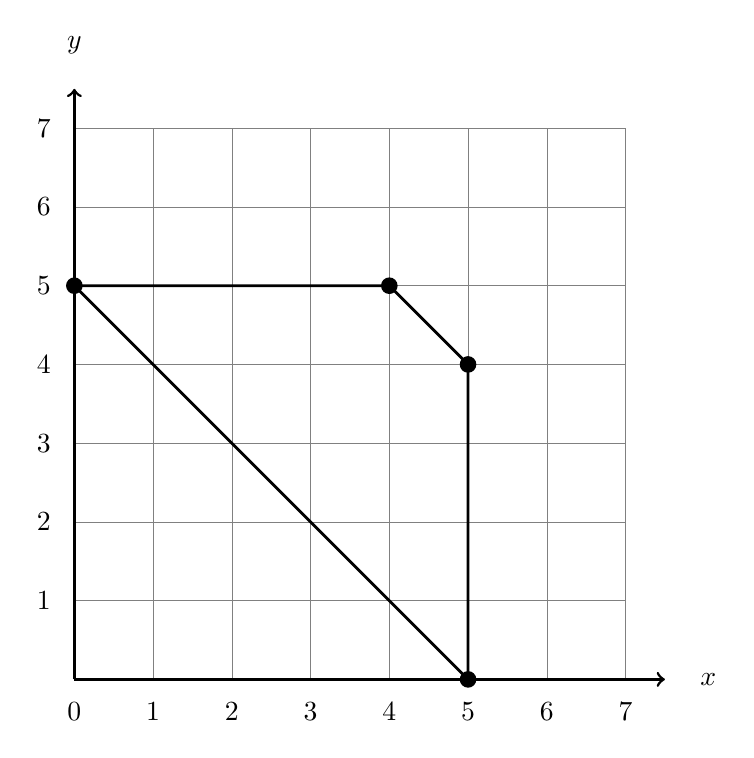
\begin{tikzpicture}
        \draw[help lines] (0,0) grid (7,7);
        \draw[->,shorten >=-5mm,line width=1pt] (0,0) -- (0,7) node[pos=1.15] {$y$};
        \draw[->,shorten >=-5mm,line width=1pt] (0,0) -- (7,0) node[pos=1.15] {$x$};
        \foreach \x in {0,...,7} {
            \node[below=5pt] at (\x,0) {$\x$};
        }
        \foreach \y in {1,...,7} {
            \node[left=5pt] at (0,\y) {$\y$};
        }
        \fill (0,5) circle (3pt);
        \fill (5,0) circle (3pt);
        \fill (4,5) circle (3pt);
        \fill (5,4) circle (3pt);
        \draw[line width=1pt] (0,5) -- (5,0) -- (5,4) -- (4,5) -- cycle;
    
    \end{tikzpicture}
\end{center}
\desarrollo[8cm]
\respuesta[3]

\pregunta Calcule el área [2 puntos] y perimetro [2 puntos] de un cuadrado con 
diagonal de largo $6\sqrt{2}$.

\begin{center}
    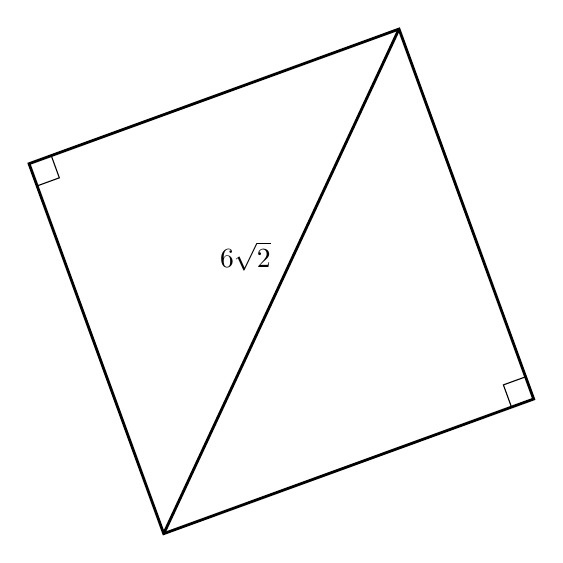
\begin{tikzpicture}[rotate=20]
        \draw[line width=1pt] (0,0) rectangle (5,5);
        \draw[] (0,5) rectangle +(0.3,-0.3);
        \draw[] (5,0) rectangle +(-0.3,0.3);
        \draw[line width=1pt] (0,0) -- (5,5) node[midway,above left] {$6\sqrt{2}$};
    \end{tikzpicture}
\end{center}

\desarrollo[8cm]
\respuesta[3]



\newpage

\parte En esta sección, de manera guiada, determinaremos el valor
de la hipotenusa para un triángulo rectángulo sin hacer uso
del teorema de Pitágoras.

\underline{Nuestra misión es:}

\begin{center}
    \begin{tikzpicture}    
        \tikzset{msg/.style={draw, dashed,line width = 1pt, text width=11cm,inner sep=10pt, rounded corners=5pt}}
        \draw [line width=1pt] (0,3) -- (0,0) -- (4,0) -- cycle;
        %\node [circle,draw,xshift=1cm,yshift=1cm] at (0,0) {\resizebox{10pt}{!}{\faStar}};
        \draw [line width=1pt] (0,0) rectangle (0.3,0.3);
        \draw[decorate, decoration={calligraphic brace,raise=4pt,amplitude=10pt}] 
            (0,0) -- (0,3) node[pos=0.5,left=15pt] {$3$};
        \draw[decorate, decoration={calligraphic brace,mirror,raise=4pt,amplitude=10pt}] 
            (0,0) -- (4,0) node[pos=0.5,below=15pt] {$4$};
        \coordinate (M) at ($(0,3)!0.5!(4,0)$);
        \node [msg, anchor=south west] (A) at ($(M)!2cm!90:(4,0)$)  {Demostrar que este lado del triángulo (la hipotenusa) mide 5};
        \draw [->, line width=1pt, shorten >=5pt] (A.south west) to[bend right=15] (M);
    \end{tikzpicture}    
\end{center}

Para demostrar esto, usaremos la siguiente figura.

\begin{center}
    \begin{tikzpicture}
        \pgfmathsetmacro{\a}{3};
        \pgfmathsetmacro{\b}{4};
    
        \draw[line width=1pt] (0,0) rectangle (\a+\b, \a+\b);
        \draw[line width=1pt] (0,\a) -- (\b,0) -- (\a + \b, \b) -- (\a,\a+\b) -- cycle;
        \draw[line width=1pt] (0,0) rectangle +(0.3,0.3);
        \draw[line width=1pt] (\a+\b,\a+\b) rectangle +(-0.3,-0.3);
        \draw[line width=1pt] (0,\a+\b) rectangle +(0.3,-0.3);
        \draw[line width=1pt] (\a+\b,0) rectangle +(-0.3,0.3);
    
        \draw[decorate, decoration={calligraphic brace,raise=4pt,amplitude=10pt}] 
            (0,0) -- (0,\a) node[pos=0.5,left=15pt] {$3$};
        \draw[decorate, decoration={calligraphic brace,raise=4pt,amplitude=10pt}] 
            (0,\a) -- (0,\a+\b) node[pos=0.5,left=15pt] {$4$};
        \draw[decorate, decoration={calligraphic brace,mirror,raise=4pt,amplitude=10pt}] 
            (\a+\b,0) -- (\a+\b,\b) node[pos=0.5,right=15pt] {$4$};
        \draw[decorate, decoration={calligraphic brace,mirror,raise=4pt,amplitude=10pt}] 
            (\a+\b,\b) -- (\a+\b,\a+\b) node[pos=0.5,right=15pt] {$3$};
        \draw[decorate, decoration={calligraphic brace,mirror,raise=4pt,amplitude=10pt}] 
            (0,0) -- (\b,0) node[pos=0.5,below=15pt] {$4$};
        \draw[decorate, decoration={calligraphic brace,mirror,raise=4pt,amplitude=10pt}] 
            (\b,0) -- (\a+\b,0) node[pos=0.5,below=15pt] {$3$};
        \draw[decorate, decoration={calligraphic brace,raise=4pt,amplitude=10pt}] 
            (0,\a+\b) -- (\a,\a+\b) node[pos=0.5,above=15pt] {$3$};
        \draw[decorate, decoration={calligraphic brace,raise=4pt,amplitude=10pt}] 
            (\a,\a+\b) -- (\a+\b,\a+\b) node[pos=0.5,above=15pt] {$4$};
        
        \node [scale=1.5,xshift=0.5cm,yshift=0.5cm] at (0,0) {$\triangle_1$};
        \node [scale=1.5,xshift=-0.5cm,yshift=0.5cm] at (\a+\b,0) {$\triangle_2$};
        \node [scale=1.5,xshift=-0.5cm,yshift=-0.5cm] at (\a+\b,\a+\b) {$\triangle_3$};
        \node [scale=1.5,xshift=0.5cm,yshift=-0.5cm] at (0,\a+\b) {$\triangle_4$};
        \node [scale=1.5] at (\a/2+\b/2,\a/2+\b/2) {$\square_5$};
    
    \end{tikzpicture}
\end{center}

% \newsavebox\mybox
% \sbox{\mybox}{<content>}
% \wd\mybox % width
% \ht\mybox % height
% \dp\mybox % depth

\NewDocumentCommand{\sT}{m}{\resizebox{15pt}{!}{$\triangle_{#1}$}}
\NewDocumentCommand{\sC}{m}{\resizebox{15pt}{!}{$\square_{#1}$}}

Donde los símbolos \sT{1}, \sT{2}, \sT{3}, \sT{4} y \sC{5} se usan para indicar 
las distintas partes que forman la figura completa.\par
\vspace{6pt}
Por último, antes de empezar la demostración, debemos recordar que:
\begin{itemize}[label=\textbullet,nosep]
    \item \underline{El área de un cuadrado} se calcula como su alto por el ancho. 
    \begin{equation*}
        \setlength{\belowdisplayskip}{0pt} \setlength{\belowdisplayshortskip}{0pt}
        \setlength{\abovedisplayskip}{0pt} \setlength{\abovedisplayshortskip}{0pt}
        A(\square) = \textrm{lado}\cdot\textrm{lado}
    \end{equation*}
    \item \underline{El área de un triángulo} se calcula como la mitad de su base 
    por la altura.
    \begin{equation*}
        \setlength{\belowdisplayskip}{0pt} \setlength{\belowdisplayshortskip}{0pt}
        \setlength{\abovedisplayskip}{0pt} \setlength{\abovedisplayshortskip}{0pt}
        A(\triangle) = \dfrac{\textrm{base}\cdot\textrm{altura}}{2}
    \end{equation*}
\end{itemize}
\vspace*{6pt} \par
Ahora, siga los pasos como se detalla a continuación.

\pregunta Calcula el área del cuadrado completo [1 punto].
\begin{center}
    \begin{tikzpicture}[x=0.5cm,y=0.5cm]
        \pgfmathsetmacro{\a}{3};
        \pgfmathsetmacro{\b}{4};
    
        \draw[line width=1pt] (0,0) rectangle (\a+\b, \a+\b);
        \draw[dashed] (0,\a) -- (\b,0) -- (\a + \b, \b) -- (\a,\a+\b) -- cycle;
        \draw[line width=1pt] (0,0) rectangle +(0.3,0.3);
        \draw[line width=1pt] (\a+\b,\a+\b) rectangle +(-0.3,-0.3);
        \draw[line width=1pt] (0,\a+\b) rectangle +(0.3,-0.3);
        \draw[line width=1pt] (\a+\b,0) rectangle +(-0.3,0.3);
    
        \draw[decorate, decoration={calligraphic brace,raise=4pt,amplitude=10pt}] 
            (0,0) -- (0,\a) node[pos=0.5,left=15pt] {$3$};
        \draw[decorate, decoration={calligraphic brace,raise=4pt,amplitude=10pt}] 
            (0,\a) -- (0,\a+\b) node[pos=0.5,left=15pt] {$4$};
        \draw[decorate, decoration={calligraphic brace,mirror,raise=4pt,amplitude=10pt}] 
            (0,0) -- (\b,0) node[pos=0.5,below=15pt] {$4$};
        \draw[decorate, decoration={calligraphic brace,mirror,raise=4pt,amplitude=10pt}] 
            (\b,0) -- (\a+\b,0) node[pos=0.5,below=15pt] {$3$};
    
    \end{tikzpicture}
\end{center}
\desarrollo[3cm]
\respuesta

\pregunta Calcula el área del triángulo \sT{1} [1 punto].
\begin{center}
    \begin{tikzpicture}    
        \tikzset{msg/.style={draw, dashed,line width = 1pt, text width=11cm,inner sep=10pt, rounded corners=5pt}}
        \draw [line width=1pt] (0,3) -- (0,0) -- (4,0) -- cycle;
        \node [xshift=1cm,yshift=1cm] at (0,0) {\sT{1}};
        \draw [line width=1pt] (0,0) rectangle (0.3,0.3);
        \draw[decorate, decoration={calligraphic brace,raise=4pt,amplitude=10pt}] 
            (0,0) -- (0,3) node[pos=0.5,left=15pt] {$3$};
        \draw[decorate, decoration={calligraphic brace,mirror,raise=4pt,amplitude=10pt}] 
            (0,0) -- (4,0) node[pos=0.5,below=15pt] {$4$};
    \end{tikzpicture}    
\end{center}
\desarrollo[3cm]
\respuesta

\pregunta Sabemos que el área de la figura completa es igual a la suma del área de 
las figuras que la forman. Es decir:

\def\cuadradoCompleto{%
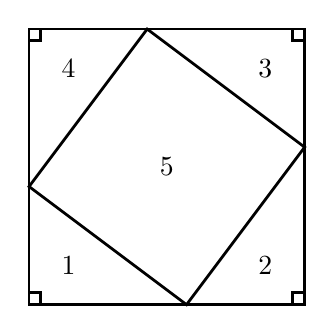
\begin{tikzpicture}[x=0.5cm,y=0.5cm]
    \pgfmathsetmacro{\a}{3};
    \pgfmathsetmacro{\b}{4};

    \draw[line width=1pt] (0,0) rectangle (\a+\b, \a+\b);
    \draw[line width=1pt] (0,\a) -- (\b,0) -- (\a + \b, \b) -- (\a,\a+\b) -- cycle;
    \draw[line width=1pt] (0,0) rectangle +(0.3,0.3);
    \draw[line width=1pt] (\a+\b,\a+\b) rectangle +(-0.3,-0.3);
    \draw[line width=1pt] (0,\a+\b) rectangle +(0.3,-0.3);
    \draw[line width=1pt] (\a+\b,0) rectangle +(-0.3,0.3);

    \node [xshift=0.5cm,yshift=0.5cm] at (0,0) {\sT{1}};
    \node [xshift=-0.5cm,yshift=0.5cm] at (\a+\b,0) {\sT{2}};
    \node [xshift=-0.5cm,yshift=-0.5cm] at (\a+\b,\a+\b) {\sT{3}};
    \node [xshift=0.5cm,yshift=-0.5cm] at (0,\a+\b) {\sT{4}};
    \node [] at (\a/2+\b/2,\a/2+\b/2) {\sC{5}};
\end{tikzpicture}}

\def\tUno{%
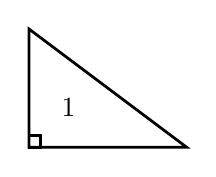
\begin{tikzpicture}[x=1cm,y=1cm,scale=0.5]
    \pgfmathsetmacro{\a}{3};
    \pgfmathsetmacro{\b}{4};
    \draw[line width=1pt] (0,0) -- (\b,0) -- (0,\a) -- cycle;
    \draw[line width=1pt] (0,0) rectangle +(0.3,0.3);
    \node [xshift=0.5cm,yshift=0.5cm] at (0,0) {\sT{1}};
\end{tikzpicture}}
\def\tDos{%
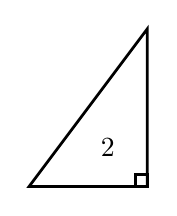
\begin{tikzpicture}[rotate=90,scale=0.5]
    \pgfmathsetmacro{\a}{3};
    \pgfmathsetmacro{\b}{4};
    \draw[line width=1pt] (0,0) -- (\b,0) -- (0,\a) -- cycle;
    \draw[line width=1pt] (0,0) rectangle +(0.3,0.3);
    \node[xshift=-0.5cm,yshift=0.5cm] at (0,0) {\sT{2}};
\end{tikzpicture}}
\def\tTres{%
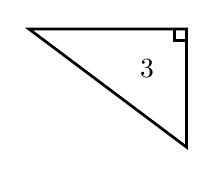
\begin{tikzpicture}[scale=0.5,rotate=180]
    \pgfmathsetmacro{\a}{3};
    \pgfmathsetmacro{\b}{4};
    \draw[line width=1pt] (0,0) -- (\b,0) -- (0,\a) -- cycle;
    \draw[line width=1pt] (0,0) rectangle +(0.3,0.3);
    \node[xshift=-0.5cm,yshift=-0.5cm] at (0,0) {\sT{3}};
\end{tikzpicture}}
\def\tCuatro{%
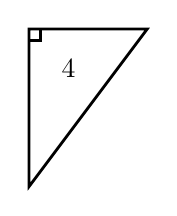
\begin{tikzpicture}[scale=0.5,rotate=270]
    \pgfmathsetmacro{\a}{3};
    \pgfmathsetmacro{\b}{4};
    \draw[line width=1pt] (0,0) -- (\b,0) -- (0,\a) -- cycle;
    \draw[line width=1pt] (0,0) rectangle +(0.3,0.3);
    \node[xshift=0.5cm,yshift=-0.5cm] at (0,0) {\sT{4}};
\end{tikzpicture}}
\def\cChico{%
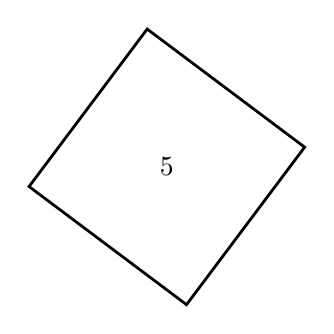
\begin{tikzpicture}[scale=0.5]
    \pgfmathsetmacro{\a}{3};
    \pgfmathsetmacro{\b}{4};
    \draw[line width=1pt] (0,\a) -- (\b,0) -- (\a + \b, \b) -- (\a,\a+\b) -- cycle;
    \node[xshift=0cm] at (\a/2+\b/2,\a/2+\b/2) {\sC{5}};
\end{tikzpicture}
}

\begin{center}
    \begin{tikzpicture}
        \node (A) {\cuadradoCompleto};
        \node [right=10pt of A.east,anchor=west] (B) {\Huge $=$};
        \node [right=10pt of B.east,anchor=west] (C) {
            \begin{tikzpicture}
                \matrix[matrix of nodes,nodes in empty cells,nodes={minimum height=30pt,minimum width=10pt,anchor=center}] (m) 
                    {   \tUno & {\Huge +} & \tDos & {\Huge +} & \tTres \\
                        \tCuatro & {\Huge +} & \cChico  & &   \\
                    };
                \end{tikzpicture}
        };
    \end{tikzpicture}
\end{center}

Además, también sabemos que los triángulos \sT{1}, \sT{2}, \sT{3} y \sT{4} son todos
iguales. Por lo cual, tienen la misma área.

Use todo esto, junto a los resultados alcanzados en (1) y (2), para 
\underline{encontrar el área del cuadrado \sC{5}} [1 punto].
\desarrollo[3cm]
\respuesta

\pregunta Si conocemos el área del cuadrado \sC{5} (pregunta anterior), 
¿Cuánto miden los lados del cuadrado \sC{5}? [1 punto]
\desarrollo[2cm]
\respuesta

{\bfseries En conclusión:} Como la hipotenusa del triángulo \sT{1} es un lado del 
cuadrado \sC{5}, hemos demostrado que para un triángulo rectángulo, con 
catetos de largo 3 y 4, la hipotenusa mide 5. En otras palabras, se cumple que:
\begin{equation*}
    3^2 + 4^2 = (\textrm{Hipotenusa})^2 \;.
\end{equation*} 

\end{document}